\chapter{Results}\label{ch:results}

Please note: this chapter is written as a demonstrator section for expediency. There has not been enough time to complete the chapter. Therefore, in my descriptions I explain the current state of the chapter. Section~\ref{sec:resindividual} has not been updated from the first test run, because I have not had time. Instead, I focused my attention on Section~\ref{sec:ressocial} because, if we have to pair down this project to meet the deadline, I believe that that section will be more relevant.

A total of 155 stories\improvement{make sure stories are explained in Chapter~\ref{ch:methods}} were identified in the interviews, excluding those pertaining to the participants' scientific field of research.

\section{Drivers and barriers to CAN science-policy engagement}\label{sec:resultsISM}

\begin{figure}[!ht]
    \centering
    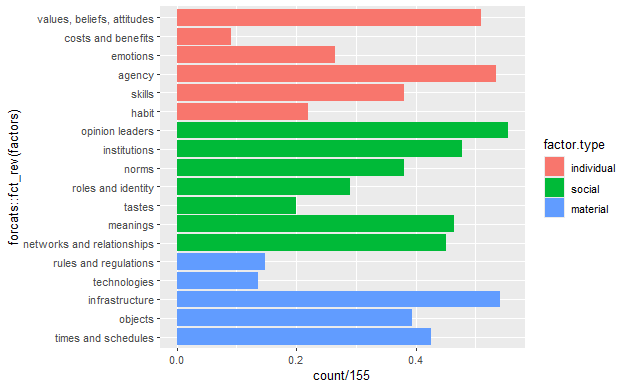
\includegraphics[width=1\linewidth]{figures/ism_count_per_story.png}
    \caption{Number of stories mentioning ISM factors}
    \label{fig:ismstorycount}
\end{figure}

The ISM framework\improvement{make sure this is explained and referenced in Chapter~\ref{ch:lit} and how I used it is described in Chapter~\ref{ch:methods}} was used to identify the behaviour factors that enable or inhibit engagement and influence at the science policy interface. Figure~\ref{fig:ismstorycount} shows the number of stories in which each factor was mentioned. Each section below describes the nature of the drivers for each of 18 behavioural factors, as identified in the interviews.


\subsection{Individual factors}\label{sec:resindividual}

Currently, this section is was the first test of the method and has not been updated. It is based on the first 6 of 18 behavioural factors and for 3 of 14 participants. It is expected (there is some evidence) that broader patterns will emerge as the analysis continues such as different `types' of scientist in regards to these different factors. The second test, in the following section~\ref{sec:ressocial}, has been applied to the interviews with all 14 participants.

\subsubsection{Values, beliefs, attitudes}\label{sec:resismvalues}
Participants stated a range of values, beliefs and attitudes that motivated them to undertake policy-relevant science and engage with policy. All indicated that their science should be \emph{useful} and, similarly, most felt that \emph{policy should be based on the best science}. One scientist has a strongly normative approach to their work, indicating that they undertook their work because they believed science should be \emph{open}, \emph{credible}, \emph{relevant} and \emph{responsible}. They also believed that they had a duty to return \emph{value for public money}. Another was more ethically-driven, indicating that they undertook their work for reasons of \emph{social justice} and that they had a \emph{duty to try}.  

\subsubsection{Costs and benefits}\label{sec:resismcab}
There was very little indication of scientists weighing up the costs and benefits of their work or that of others. One scientist balanced the value of their activity with its used for policymaking and concluded that \emph{it's worth it} - ``\emph{If it's going to be useful, why wouldn't we prioritise our time to do that paper rather than something else\index{p01}}'', this was linked to an acknowledgement of the costs and benefits to policymakers for whom reading all the relevant scientific literature is \emph{too much effort}. Regarding engaging at the science policy interface, another scientist felt that they were \emph{not sure its worth the effort} - ``\emph{I'm not convinced that it overall is hugely impactful\index{p03}}''.

\subsubsection{Emotions}\label{sec:resismemotions}
Various emotions were associated with undertaking science and engaging with policy including \emph{exhaustion}, \emph{intrigue}, \emph{pleasure} and \emph{pride}. However, these were largely expressed only by one participant, with another expressing no emotions.

\subsubsection{Agency}\label{sec:resismagency}
Agency was, by far, the most commonly expressed driver or barrier to working on policy-related science and engaging with policy. There was a contrast between one scientist who frequently expressed confidence in \emph{making it happen} alongside being \emph{open to new ideas}. This contrasted with another participant who was more likely to express \emph{limits to my influence}. Most participants also noted the role of \emph{happenstance} in their ability to engage at the science policy interface. The agency of others were also noted by participants, such as the ability of NGOs in terms of \emph{making it happen} and that policymakers and stakeholders in policy (such as businesses) could be \emph{open to new ideas}.

\subsubsection{Skills}\label{sec:resismskills}
Understandably, skills were also identified as important for engaging with policy. In particular statements indicating that engagement was possible because scientists \emph{know and understand the science} and also when scientists \emph{know and understand how policy is made}. Further, participants identified that how well policymakers \emph{know and understand the science} affected engagement (if they don't know and understand, they would reach out to scientists) but also how well policy is made (if they don't know and understand the science, they can choose poor evidence for decisionmaking).

\subsubsection{Habit}\label{sec:resismhabit}
Two habits were identified within the interviews. The first, identified by all participants was the habit of \emph{scientists doing science for scientists} which tended to be less useful for policymaking. The other habit, which participants often, but not always, identified as a barrier to engagement was \emph{policy obtaining information from the same sources} rather than reaching out to scientists with more policy-challenging perspectives. This was less of a barrier in the context that scientists used this knowledge to publish their work in media deemed to be popular with policymakers.

\subsection{Social factors}\label{sec:ressocial}

This section demonstrates the second test of the method and synthesises the interviews of all 14 participants. Because Figure~\ref{fig:ismstorycount} indicates that social factors are more `important' than individual or material factors, I have focused on these.

Each section describes the results for one factor. The section includes a table which outlines each type of mention for that factor, whether the factor enabled/inhibited engagement or influence, and an example quote from the interviews. A short description of these mentions is given, followed by typical strategies applied by scientists which either exploits or counteracts the factor.

\subsubsection{Opinion leaders}\label{sec:resopinionleaders}

\begin{table}[!ht]
\footnotesize
\caption{The 7 types of mention of \emph{opinion leaders} in the interviews and example quotes for each type}\label{tab:resopinionleaders}
%\begin{tabularx}{\textwidth} {DIQ} 
\begin{tabular}{p{.08\linewidth}p{.3\linewidth}p{.1\linewidth}p{.42\linewidth}}\hline
\textbf{id} & \textbf{mention type} & \textbf{influence} & \textbf{quote} \\ \hline \hline 
ol1 & scientists' knowledge   drew interest from policymakers & enabler & ``They had already decided they wanted to   work with us''\index{p05}  \\[5mm]
ol2 & scientists influencing policymakers & enabler & ``Informally I think they [have been] picked up and had a bit of   traction''\index{p03}  \\[5mm]
ol3 & scientists influencing others & enabler & ``We've been cited by both industry and NGOs on different sides of   the debate, so we've probably got something right there''\index{p01} \\[5mm]
ol4 & senior scientists are more likely to be   listened to & enabler & ``When it comes to something for more formal like that, they tend to   go for the professors''\index{p03} \\[5mm]
ol5 & I look up to other scientists & enabler & ``He's an excellent scientist, he's very inclusive and he's   incredibly motivational from a scientific perspective, very much in favour of   community building''\index{p04} \\[5mm]
ol6 & others influence policymakers & inhibitor & ``Sometimes what they bring is politically convenient, and   policymaking is not just about evidence is also about political convenience   or political opportunity. They provide narratives to use or discard certain   evidence.''\index{p09}  \\[5mm]
ol7 & policymakers have influence & neutral & ``I think policy makers have the greatest leverage of   all''\index{p08}  \\[5mm] \hline
ols1 & opportunities to promote my/our work & enabler & ``If I get media requests, I think if I've got the expertise, I   should do that because it goes with the job''\index{p01}  \\[5mm]
ols2 &  opportunities to understand the perspectives of policymakers & enabler & ``we try and find out what their priorities are''\index{p12} \\[5mm] \hline
\end{tabular}
%\end{tabularx}
\end{table}
\improvement{the layout of this table needs to be easier to read}

Nearly half of the stories mention individuals and groups to whom scientists and policymakers will reach out, and be influenced by, more than any other social factor. This indicates that opinion leaders are important to scientists engaging with policy. Given the criteria for inviting people to take part in this study, it is not surprising that many participants mentioned being invited by policymakers to share their knowledge (ol1). Others identified that they believed they had had some influence on policymaking (ol2) or others, such as industry and NGOs (ol3). The was specific recognition that senior scientists are more likely to have influence (ol4).  

It was also quite common to observe that there are non-science actors, such as other governments, industry, learned societies, research councils, special advisers and NGOs, who have influence in the decisions being make (ol6). Further, policymakers themselves were considered to have influence (ol7)

\paragraph{Strategies:}

In some cases, this understanding has been used to gain influence. A number of participants mentioned promoting their work through third parties such as media opportunities but also by engaging with organisations such as industry or NGOs such as charities, campaigning organisations and networks (think tanks) as a mechanism for influencing policymaking (ols1). A different approach was to make efforts to align with policymakers by taking up opportunities to listen to their perspectives (ols2).

\subsubsection{Institutions}\label{sec:resinstitutions}
\subsubsection{Norms}\label{sec:resnorms}
\subsubsection{Roles and identity}\label{sec:resroles}

\begin{table}[!ht]
\footnotesize
\caption{The \emph{roles} and \emph{identities} of scientists expressed in the interviews}\label{tab:resopinionleaders}
%\begin{tabularx}{\textwidth} {DIQ} 
\begin{tabular}{p{.45\linewidth}p{.45\linewidth}}\hline
\textbf{roles} & \textbf{identities} \\ \hline\hline
academic, adviser, advocate, citizen, public servant, representative, researcher, specialist & authoritative, candid, esteemed, experienced, expert, helpful, humble, impartial, informed, judicious, receptive, relevant \\[5mm] \hline
role conflicts: researcher versus adviser, adviser versus advocate & deserving recognition \\[5mm] \hline
\end{tabular}
%\end{tabularx}
\end{table}



There was were other roles noted in reference to others, such a politician, civil servant

\subsubsection{Tastes}\label{sec:restastes}
\subsubsection{Meanings}\label{sec:resmeanings}
\subsubsection{Network and relationships}\label{sec:resnetwork}
\subsection{Material factors}\label{sec:resmaterial}
\subsubsection{Rules and regulations}\label{sec:resrules}
\subsubsection{Technologies}\label{sec:restechnologies}
\subsubsection{Objects}\label{sec:resobjects}
\subsubsection{Infrastructure}\label{sec:resinfrastructure}
\subsubsection{Times and schedules}\label{sec:restimes}

\section{General notes}
By nature, participants are people who respond to requests to provide information

%Passion for their subject evident across participants
%Keen for policy to use best knowledge and feel they have that knowledge
%Evidence of awareness of policy cycle? P5
%Comments on political context and/or change of government
%Involvement of other organisations - industry, NGOs, civil society, citizens?

%
